% Avance 1 · Detección de celdas solares defectuosas en imágenes EL · PDI 2026-III
% Compilar con XeLaTeX desde esta carpeta:  latexmk -xelatex informe.tex
% Todas las figuras y cifras salen de los scripts del repo (ver la sección "Reproducir").
\documentclass[11pt,a4paper]{article}

\usepackage{fontspec}
\usepackage[spanish,es-noshorthands,es-nodecimaldot,es-tabla]{babel}
\usepackage[a4paper,top=2.3cm,bottom=2.3cm,left=2.4cm,right=2.4cm,headheight=14pt]{geometry}
\usepackage{amsmath,amssymb}
\usepackage{graphicx}
\usepackage{booktabs,array,tabularx,multirow}
\usepackage[table]{xcolor}
\usepackage[most]{tcolorbox}
\usepackage{fancyhdr}
\usepackage{enumitem}
\usepackage{caption}
\usepackage{float}
\usepackage{placeins}
\usepackage[hidelinks]{hyperref}

\graphicspath{{../../reports/figures/}{../comun/}}

\definecolor{ud}{RGB}{128,57,61}
\definecolor{udsoft}{RGB}{242,230,231}
\definecolor{tinta}{RGB}{50,50,50}
\definecolor{gris}{RGB}{120,120,120}
\definecolor{okc}{RGB}{27,140,96}

\captionsetup{font=small,labelfont={bf,color=ud},labelsep=period}
\setlist{itemsep=2pt,topsep=4pt}
\setlength{\parskip}{4pt}
\setlength{\parindent}{0pt}

\pagestyle{fancy}\fancyhf{}
\fancyhead[L]{\small\color{gris}Celdas solares defectuosas en imágenes EL}
\fancyhead[R]{\small\color{gris}Avance 1 · PDI 2026-III}
\fancyfoot[C]{\small\color{gris}\thepage}
\renewcommand{\headrulewidth}{0.3pt}

\newtcolorbox{decision}[1]{enhanced,breakable,colback=udsoft,colframe=ud,boxrule=0.6pt,arc=1pt,
  left=6pt,right=6pt,top=4pt,bottom=4pt,fonttitle=\bfseries\small,coltitle=white,title={#1}}
\newtcolorbox{ojo}[1]{enhanced,breakable,colback=white,colframe=ud,boxrule=0.6pt,arc=1pt,
  borderline west={3pt}{0pt}{ud},left=8pt,right=6pt,top=4pt,bottom=4pt,
  fontupper=\small,title={#1},fonttitle=\bfseries\small,coltitle=ud,colbacktitle=white,attach title to upper={\quad}}

\newcommand{\hecho}{{\color{okc}$\checkmark$}}
\newcommand{\cifra}[2]{\begin{minipage}[t]{0.235\textwidth}\centering{\color{ud}\fontsize{20}{22}\selectfont #1}\par\vspace{2pt}{\footnotesize #2}\end{minipage}}

\begin{document}

% ------------------------------------------------------------------ portada compacta
\begin{minipage}[c]{0.14\textwidth}
\includegraphics[width=\linewidth]{logo.png}\end{minipage}\hfill
\begin{minipage}[c]{0.83\textwidth}
  {\small\color{gris}Procesamiento Digital de Imágenes · Universidad Distrital Francisco José de Caldas}\par\vspace{3pt}
  {\LARGE\color{ud}Avance 1 · Datos, partición y línea base}\par\vspace{3pt}
  {\large Detección de celdas solares defectuosas en imágenes de electroluminiscencia}\par\vspace{4pt}
  {\small Joel Eduardo Reyes Barrios (20212005011) · Johan Sebastián Cáceres Rodríguez (20212005111) ·
   Hosman Javier Nieto Cruz (20212005117)}\par
  {\small\color{gris}Semana 1 del cronograma (9 – 15 de noviembre de 2026)}
\end{minipage}
\vspace{6pt}
{\color{ud}\rule{\textwidth}{0.8pt}}

% ------------------------------------------------------------------ 1
\section*{1 \quad Resumen}

La semana 1 dejó lista la base sobre la que se mide todo lo demás. Reconstruimos los 44 paneles de ELPV, partimos los datos
\textbf{por panel} y comprobamos que no hay fuga. También medimos la primera versión de la máscara y de la normalización,
medimos la línea base del sistema en validación y dejamos la GPU lista para la CNN.

\vspace{4pt}
\noindent
\cifra{0 \textit{vs.} 498}{pares casi idénticos ($r>0{,}95$) entre partes: nuestra partición frente a una al azar}\hfill
\cifra{12\,\% → 4\,\%}{variación entre paneles del brillo de las celdas sanas, antes y después de normalizar}\hfill
\cifra{0,78}{AUC de la línea base en validación (mono 0,84 · poly 0,71)}\hfill
\cifra{7 s}{por época de la CNN en la GPU (GTX 1650, 4 GB)}
\vspace{6pt}

\begin{decision}{Lo que decidimos esta semana}
\begin{itemize}[leftmargin=12pt]
  \item \textbf{Máscara v1.} Si la máscara por brillo cubre menos del 90\,\% de la plantilla del tipo, se usa la plantilla.
        Corrige 17 celdas casi apagadas a las que la máscara les dejaba fuera justamente la zona dañada.
  \item \textbf{El brillo crudo no entra a la red.} Encontramos que los paneles con más defectos se fotografiaron más oscuros, así que el brillo crudo
        es en parte un atajo hacia el panel. La CNN solo verá imágenes normalizadas, como dice la propuesta, y la línea base se reporta con y sin esa variable.
\end{itemize}
\end{decision}

% ------------------------------------------------------------------ 2
\section*{2 \quad Avance frente al cronograma}

\begin{table}[!htbp]
\centering\small
\begin{tabularx}{\textwidth}{@{}c X >{\footnotesize}p{7.6cm}@{}}
\toprule
 & Actividad de la semana 1 (tabla 6 de la propuesta) & Dónde quedó \\
\midrule
\hecho & Descarga y análisis del conjunto & \texttt{docs/01\_dataset.md}, \texttt{docs/02\_eda.md}, \texttt{notebooks/01\_EDA.ipynb} \\
\hecho & Reconstrucción de paneles y partición & \texttt{data/particion.csv} (congelada), \texttt{docs/03\_particion.md} \\
\hecho & Primera versión de máscara y normalización & \texttt{src/preproc.py},\newline \texttt{scripts/05\_medir\_mascara\_normalizacion.py} \\
\hecho & Preparación de la GPU & \texttt{torch} 2.14 + CUDA en la GTX 1650; prueba de 3 épocas \\
\midrule
+ & Línea base medida en validación, por tipo de celda & \texttt{scripts/02\_evaluar\_caracteristicas.py} \\
\bottomrule
\end{tabularx}
\end{table}

Las cuatro actividades de la semana 1 están completas. Además adelantamos la medición de la línea base, que será la referencia que la CNN tiene que superar en la semana 3.

% ------------------------------------------------------------------ 3
\section*{3 \quad Métodos}

\paragraph{Paneles y partición.} ELPV no dice de qué panel sale cada celda. Lo reconstruimos con el orden de las imágenes, el tipo de celda, los saltos de brillo entre
paneles y el tamaño típico de 60 celdas. Así salieron 44 paneles: 18 mono y 26 poly. Encontramos además 5 pares de \emph{paneles gemelos}, que son el mismo
panel fotografiado dos veces, y van siempre juntos. La unidad que no se divide es el grupo (35 grupos). Validación y prueba reciben cada una cerca del 15\,\% de
las celdas de cada tipo. Entre 300.000 asignaciones al azar (semilla 2026) elegimos la que mejor conserva la mezcla de las cuatro etiquetas.

\paragraph{Control de fuga.} Contamos los pares de celdas casi idénticas (correlación $r>0{,}95$) que caen en partes distintas, y comparamos con una partición
al azar por celda. Es la prueba que la propuesta fijó (§5.1).

\paragraph{Máscara (v1).} Se suaviza la celda ($\sigma=3$) y se umbraliza a la mitad de su percentil 90. Después se aplica un cierre de $31\times31$, se toma la
componente conexa mayor y su envolvente convexa, y se erosiona con $17\times17$. Por último se interseca con la plantilla del tipo (mono o poly), que se
calcula \emph{solo con entrenamiento}. El cambio de esta semana es un \textbf{respaldo}:
\begin{equation}
M \;=\;
\begin{cases}
M_{\text{brillo}} \cap T_{\text{tipo}} & \text{si } |M_{\text{brillo}} \cap T_{\text{tipo}}| \ge 0{,}9\,|T_{\text{tipo}}|,\\[2pt]
T_{\text{tipo}} & \text{si no.}
\end{cases}
\end{equation}
ELPV ya trae las celdas recortadas y alineadas, así que la plantilla geométrica es una máscara válida cuando el brillo no alcanza para separar la celda.

\paragraph{Normalización.} Igual que en la propuesta (ec. 1): $I_n(x,y)=I(x,y)\,/\,P_{90}\{I(p):p\in M\}$.
Para medirla usamos solo las celdas \emph{sanas} (etiqueta 0\,\%) de los paneles de entrenamiento y validación con al menos 5 de ellas (35 paneles).
Comparamos la dispersión entre paneles de su brillo, antes y después, con el coeficiente de variación de las medianas por panel.

\paragraph{Línea base.} Usamos el pipeline heredado: busbars por cierre, dedos por cierre corto, mapa de déficit y mapa de crestas de Sato. De ahí salen 10
características por celda, más el número de busbars y el tipo. Con ellas entrenamos una regresión logística con pesos por clase, en entrenamiento, y la
medimos en validación. \textbf{No es el sistema final}: es la referencia que la CNN debe superar.

\paragraph{GPU.} Usamos una NVIDIA GTX 1650 (4 GB) con \texttt{torch} 2.14.1 + CUDA 13.0. La prueba fue la CNN de la plantilla
(\texttt{scripts/04\_entrenar\_cnn.py}), entrenada 3 épocas sobre las 1.790 celdas de entrenamiento a $128\times128$.

% ------------------------------------------------------------------ 4
\section*{4 \quad Resultados}

\FloatBarrier
\subsection*{4.1 \quad La partición no tiene fuga}

\begin{figure}[!htbp]
\centering
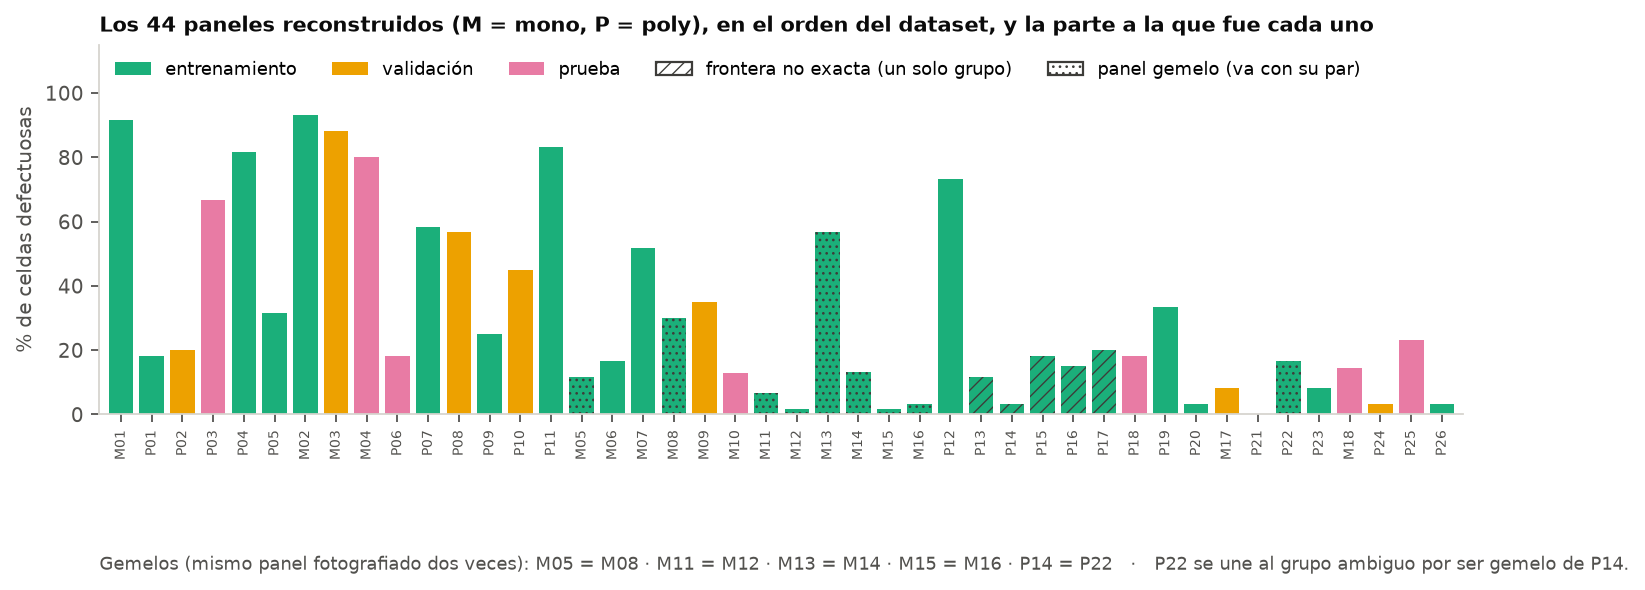
\includegraphics[width=0.84\textwidth]{p2_paneles_particion.png}
\caption{Los 44 paneles reconstruidos y la parte a la que fue cada uno. Las barras punteadas son paneles gemelos, que van con su par.}
\end{figure}

\begin{table}[!htbp]
\centering\small\setlength{\tabcolsep}{4.5pt}
\begin{tabular}{@{}l rrrrr@{}}
\toprule
Parte & Paneles & Celdas & Mono & Poly & \% def. \\
\midrule
Entrenamiento & 30 & 1.790 & 720 & 1.070 & 29,5 \\
Validación    &  7 &   432 & 192 &   240 & 35,9 \\
Prueba        &  7 &   402 & 162 &   240 & 34,3 \\
\bottomrule
\end{tabular}
\hfill
\begin{tabular}{@{}l rr@{}}
\toprule
Pares entre partes & Por panel & Al azar \\
\midrule
$r>0{,}95$ (1.193 pares) & \textbf{0} & 498 \\
$r>0{,}90$ (4.118 pares) & 7 & 1.769 \\
\bottomrule
\end{tabular}
\caption{Izquierda: composición de la partición. Derecha: pares de celdas casi idénticas que quedan en partes distintas.}
\end{table}

Con una partición al azar por celda, 498 pares casi idénticos quedarían repartidos entre partes, y el modelo podría acertar reconociendo el panel. Con la
partición por panel no queda ninguno con $r>0{,}95$. La reconstrucción de paneles funcionó.

\FloatBarrier
\subsection*{4.2 \quad La normalización iguala los paneles}

\begin{figure}[!htbp]
\centering
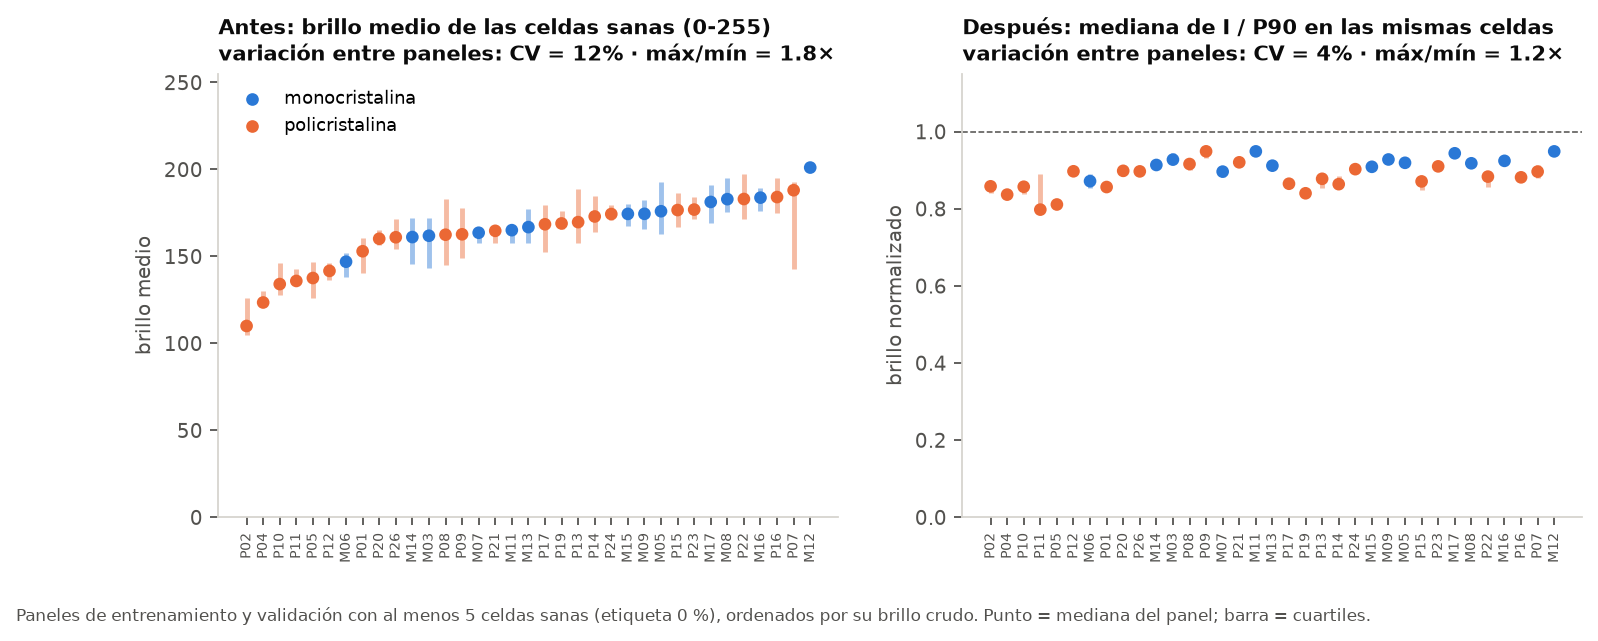
\includegraphics[width=0.84\textwidth]{n1_normalizacion_paneles.png}
\caption{Brillo de las celdas sanas de cada panel antes (izquierda) y después (derecha) de dividir por su percentil 90. Punto: mediana del panel. Barra: cuartiles.}
\end{figure}

\begin{table}[!htbp]
\centering\small
\begin{tabular}{@{}l cc cc@{}}
\toprule
 & \multicolumn{2}{c}{Variación entre paneles (CV)} & \multicolumn{2}{c}{Panel más brillante / más oscuro} \\
\cmidrule(lr){2-3}\cmidrule(lr){4-5}
 & antes & después & antes & después \\
\midrule
Todas & 11,6\,\% & \textbf{4,1\,\%} & 1,83× & \textbf{1,19×} \\
Mono  &  7,6\,\% & 2,2\,\% & & \\
Poly  & 12,7\,\% & 4,0\,\% & & \\
\bottomrule
\end{tabular}
\caption{Dispersión entre 35 paneles del brillo de sus celdas sanas.}
\end{table}

Antes de normalizar, la celda sana típica de un panel brilla hasta 1,8 veces más que la de otro. Después, las medianas de todos los paneles quedan entre
0,80 y 0,95 de su referencia, y la variación entre paneles cae a un tercio. Lo que queda (4\,\%) es mayor en poly que en mono, lo que es coherente con la
textura del grano.

\FloatBarrier
\subsection*{4.3 \quad La máscara v1 recupera las celdas casi apagadas}

\begin{figure}[!htbp]
\centering
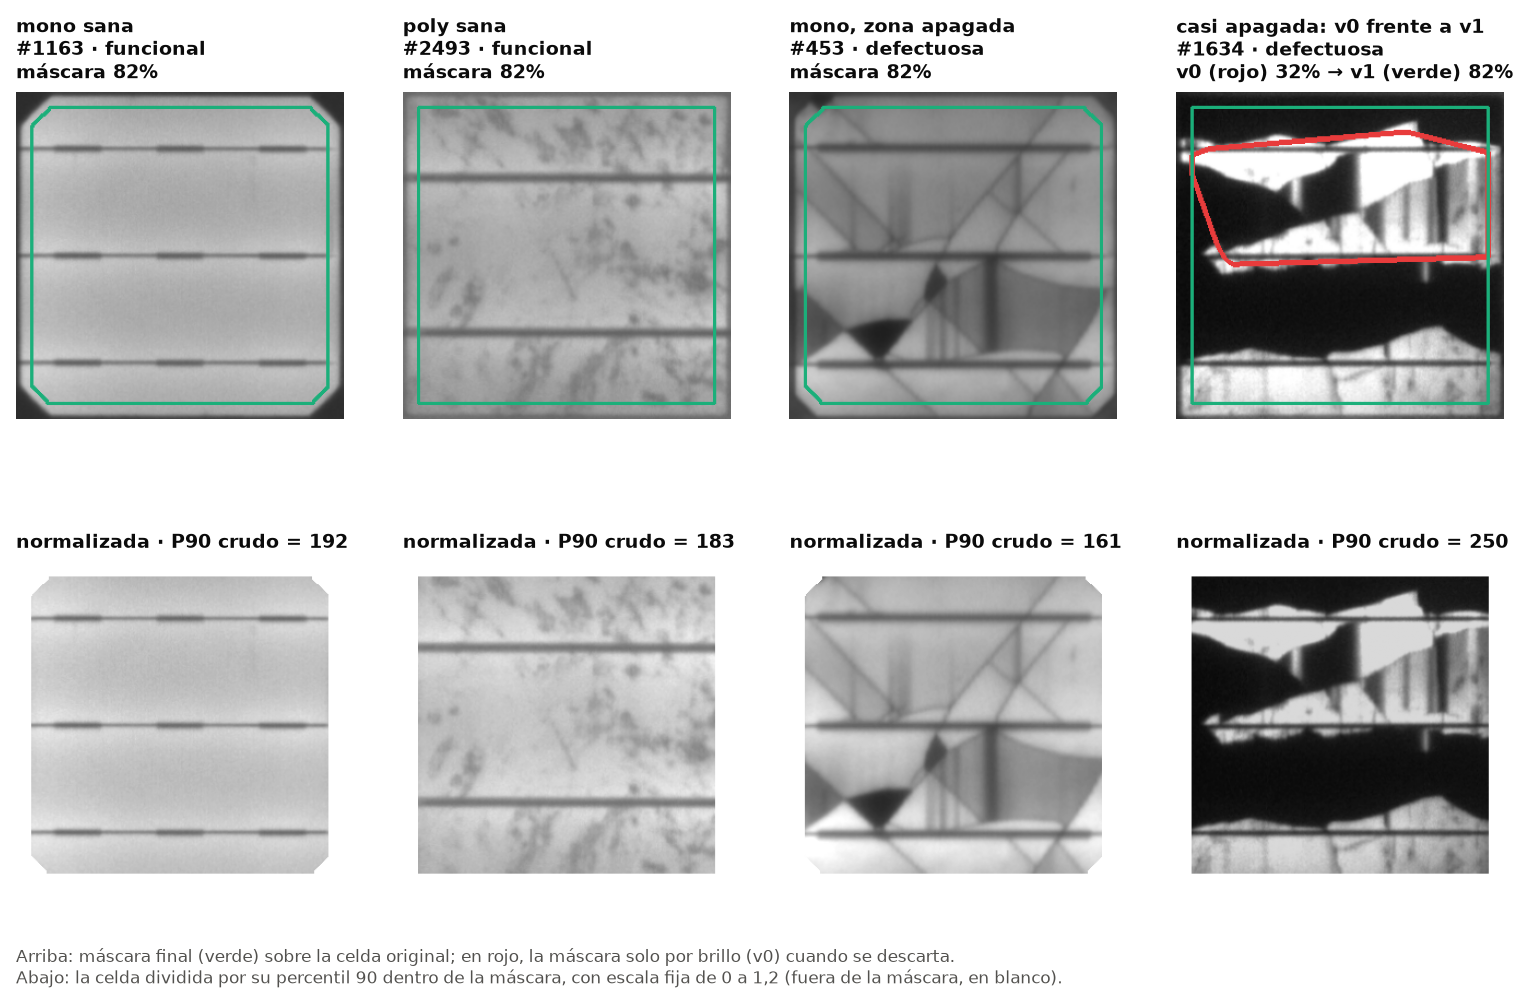
\includegraphics[width=0.68\textwidth]{n2_mascara_ejemplos.png}
\caption{Máscara final (verde) y celda normalizada en cuatro casos. En la última, la máscara solo por brillo (rojo) cubría el 32\,\% de la celda y dejaba
fuera la zona apagada; con el respaldo cubre el 82\,\%.}
\end{figure}

En el 90\,\% de las celdas, la máscara por brillo coincide exactamente con la plantilla del tipo; en el resto, la diferencia está en los bordes. Solo en
\textbf{17 celdas, todas poly, todas defectuosas y todas de entrenamiento}, la máscara se encoge más de un 10\,\%. En ellas la zona apagada es tan grande que el umbral la saca de la máscara: el mapa de déficit no podría verla y la normalización tomaría como
referencia solo la parte sana. Con el respaldo, la máscara más pequeña pasa del 32\,\% al 74\,\% de la celda. Como las 17 son de entrenamiento, la línea base
en validación no cambia.

\FloatBarrier
\subsection*{4.4 \quad Hallazgo: el brillo crudo es en parte un atajo hacia el panel}

\begin{figure}[!htbp]
\centering
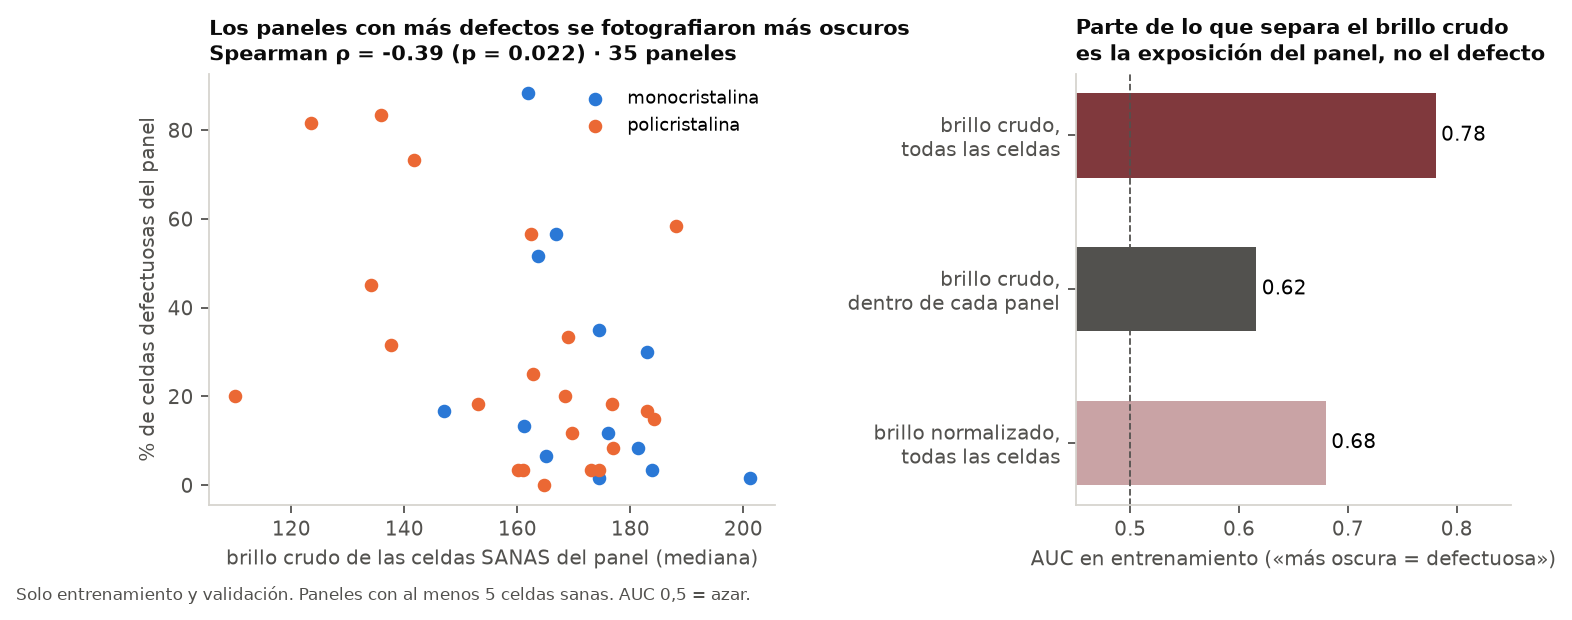
\includegraphics[width=0.84\textwidth]{n3_brillo_atajo_panel.png}
\caption{Izquierda: en ELPV, los paneles con más celdas defectuosas tienden a tener celdas sanas más oscuras. Derecha: AUC de «más oscura = defectuosa» en entrenamiento.}
\end{figure}

El brillo crudo separa las clases con AUC 0,78, pero dentro de un mismo panel solo con 0,62. La diferencia viene de la exposición: los paneles más dañados se
fotografiaron más oscuros (Spearman $\rho=-0{,}39$, $p=0{,}022$, 35 paneles). Un modelo que use el brillo crudo aprende en parte «este panel es oscuro», y eso
no es un defecto ni sirve con otra cámara. Es la razón de fondo para normalizar antes de la red.

\FloatBarrier
\subsection*{4.5 \quad Línea base en validación}

\begin{figure}[H]
\centering
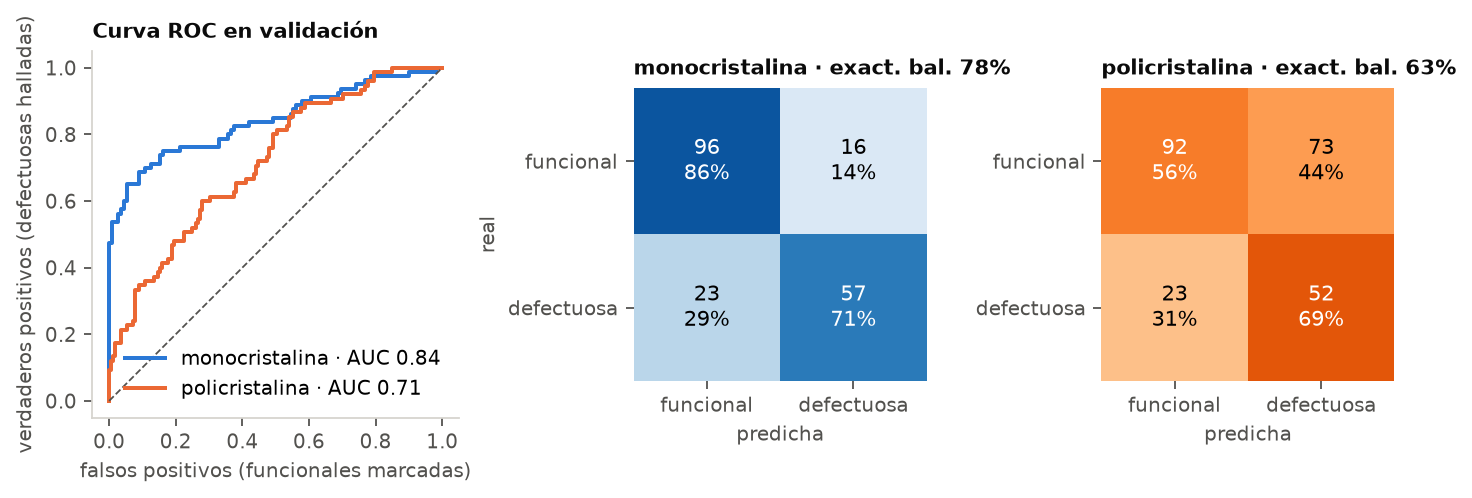
\includegraphics[width=0.86\textwidth]{f4_linea_base_val.png}
\caption{Línea base (características del pipeline + regresión logística), entrenada en entrenamiento y medida en validación.}
\end{figure}

\begin{table}[H]
\centering\small
\begin{tabular}{@{}l ccc c ccc@{}}
\toprule
 & \multicolumn{3}{c}{Con brillo crudo} & & \multicolumn{3}{c}{Sin brillo crudo} \\
\cmidrule(lr){2-4}\cmidrule(lr){6-8}
 & AUC & Exact. bal. & F1 def. & & AUC & Exact. bal. & F1 def. \\
\midrule
Mono (192 celdas) & 0,84 & 78,5\,\% & 0,75 & & 0,78 & 66,3\,\% & 0,64 \\
Poly (240 celdas) & 0,71 & 62,5\,\% & 0,52 & & 0,67 & 65,7\,\% & 0,53 \\
Todas (432)       & \textbf{0,78} & 69,1\,\% & 0,62 & & 0,73 & 67,3\,\% & 0,59 \\
\bottomrule
\end{tabular}
\caption{Métricas de la línea base en validación. El clasificador que siempre responde «funcional» tiene exactitud balanceada de 50\,\%.}
\end{table}

\begin{itemize}[leftmargin=14pt]
  \item \textbf{Mono va bien y poly no.} En poly, 73 de las 165 celdas funcionales salen marcadas como defectuosas: el filtro de crestas responde a los bordes
        de grano. Es el problema que anticipó la propuesta (§3.3).
  \item \textbf{Sin el brillo crudo el AUC baja 5 puntos}, sobre todo en mono. Parte de lo que «sabe» la línea base es la exposición del panel.
  \item \textbf{Contexto, no meta.} El artículo de referencia reporta 88,42\,\% con CNN y 82,44\,\% con SVM [1], pero con partición al azar por celda. Antes,
        con una partición al azar, esta misma línea base daba AUC 0,84. La caída a 0,78 es el precio de medir con paneles no vistos.
\end{itemize}

% ------------------------------------------------------------------ 5
\FloatBarrier
\section*{5 \quad Decisiones y cambios respecto a la propuesta}

\begin{table}[!htbp]
\centering\small
\begin{tabularx}{\textwidth}{@{}>{\raggedright}p{4.2cm} X@{}}
\toprule
Decisión & Por qué \\
\midrule
Máscara v1 con respaldo de plantilla & 17 celdas perdían su zona apagada. Es un ajuste dentro de §4.1, no cambia el método. \\
Línea base reportada con y sin brillo crudo & El brillo crudo arrastra la exposición del panel (§4.4). La CNN no lo recibe, como ya decía la propuesta. \\
Métricas balanceadas y por tipo desde ya & Validación tiene más defectuosas (36\,\%) que entrenamiento (30\,\%), porque los paneles no se pueden partir. \\
\bottomrule
\end{tabularx}
\end{table}

\textbf{Ningún cambio al alcance ni a los objetivos.} La partición sigue congelada y el conjunto de prueba no se ha usado.

% ------------------------------------------------------------------ 6
\section*{6 \quad Problemas y riesgos}

\begin{itemize}[leftmargin=14pt]
  \item \textbf{Los granos de poly.} Es el riesgo principal y ya se ve en la línea base: exactitud balanceada de 63\,\% en poly frente a 78\,\% en mono.
        Plan: Gabor y filtrado por orientación y longitud en la semana 3.
  \item \textbf{Falsos busbars.} En la línea base, una mancha oscura grande se detecta como busbar y el cierre la rellena a medias (figura \texttt{f2} del repo).
        Se corrige en la semana 2, exigiendo que la banda sea fina y abarque todo el ancho.
  \item \textbf{Celdas con dos busbars} (un grupo de poly). La detección por perfil de filas ya cuenta 2 o 3. Hay que verificar el notch en esas celdas.
  \item \textbf{Memoria de la GPU} (4 GB). Alcanza para la CNN pequeña con lotes de 32 a $128\times128$. Si se cambia a una red más grande, se usa Colab.
\end{itemize}

% ------------------------------------------------------------------ 7
\section*{7 \quad Plan de la semana 2: busbars}

\begin{enumerate}[leftmargin=16pt]
  \item \textbf{Detección de busbars} por el perfil de filas de $I_n$: número, posición y grosor, exigiendo banda fina y de todo el ancho.
  \item \textbf{A · Notch gaussiano} (ec. 2 de la propuesta), en dos variantes: en toda la celda y limitado a las filas de los busbars.
  \item \textbf{B · Cierre morfológico} (ec. 3), solo en las filas detectadas.
  \item \textbf{Dedos}: cierre horizontal corto, con revisión aparte de las grietas verticales finas.
  \item \textbf{Comparación en validación} con los criterios de imagen de la tabla 3: brillo residual en las filas del busbar, cambio fuera de ellas y tiempo
        por celda. El criterio que decide, el AUC de la CNN, se mide en la semana 3.
\end{enumerate}

% ------------------------------------------------------------------ reproducir y referencias
\vspace{4pt}
\begin{ojo}{Reproducir.}
Desde la raíz del repo, con el entorno de \texttt{requirements.txt}, se corren en orden
\texttt{scripts/01\_preprocesar\_todo.py}, \texttt{scripts/02\_evaluar\_caracteristicas.py} y
\texttt{scripts/05\_medir\_mascara\_normalizacion.py}. Las cifras quedan en \texttt{reports/metricas/} y las figuras en
\texttt{reports/figures/}. Etiqueta git: \texttt{avance-1}.
\end{ojo}

{\small
\textbf{Referencias.}
[1] S. Deitsch \emph{et al.}, «Automatic classification of defective photovoltaic module cells in electroluminescence images», \emph{Solar Energy}, vol. 185,
pp. 455–468, 2019. ·
[2] ZAE Bayern, «elpv-dataset», \texttt{github.com/zae-bayern/elpv-dataset}. Imágenes con licencia CC BY-NC-SA 4.0.
}

\end{document}
